\clearpage
\setcounter{page}{1}

\begin{center}
\title{\LARGE \bf Chapter 4}\\
\title{\LARGE \bf Pengelolaan File CSV}\\
\end{center}

\appendix
\section{Teori}

\begin{enumerate}
\item Fungsi, Sejarah, dan Contoh File CSV\\
Comma Separated Value (CSV) merupakan format yang digunakan untuk merepresentasi sekumpulan sequen. File CSV digunakan untuk membuat Database Relasional dalam bentuk spreadsheet. Format data setiap record dipisahkan dengan menggunakan tanda koma(,) atau juga bisa dengan menggunakan titik koma(;). CSV digunakan untuk bertukar informasi antara mesin dan dua arsitektur.\\

\item Aplikasi yang dapat membuat file CSV
\begin {enumerate}
\item Microsoft Excel
\item Spreadsheet
\item Text Editor (Wordpad, Notepad, dll)
\end{enumerate}

\item  Cara Menulis dan Membaca File CSV di Excel atau Spreadsheet\\
\begin{enumerate}
\item Buka dokumen baru pada Microsoft.
\item Input judul kolom untuk setiap informasi yang akan ditampilkan.\\
Contoh : NPM, Nama, Jurusan, Kelas. Lalu ketikan field dalam kolom sesuai judulnya.\\
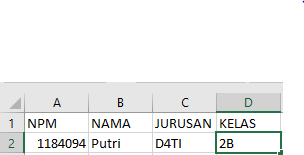
\includegraphics{gambar/csv1.png}
\item Setelah mengetikkan data pada excel, lalu pilih menu file, lalu pilih menu export, kemudian pilih menu change file type, pilih csv, lalu klik tombol save as. Maka file excel akan menjadi file csv.\\
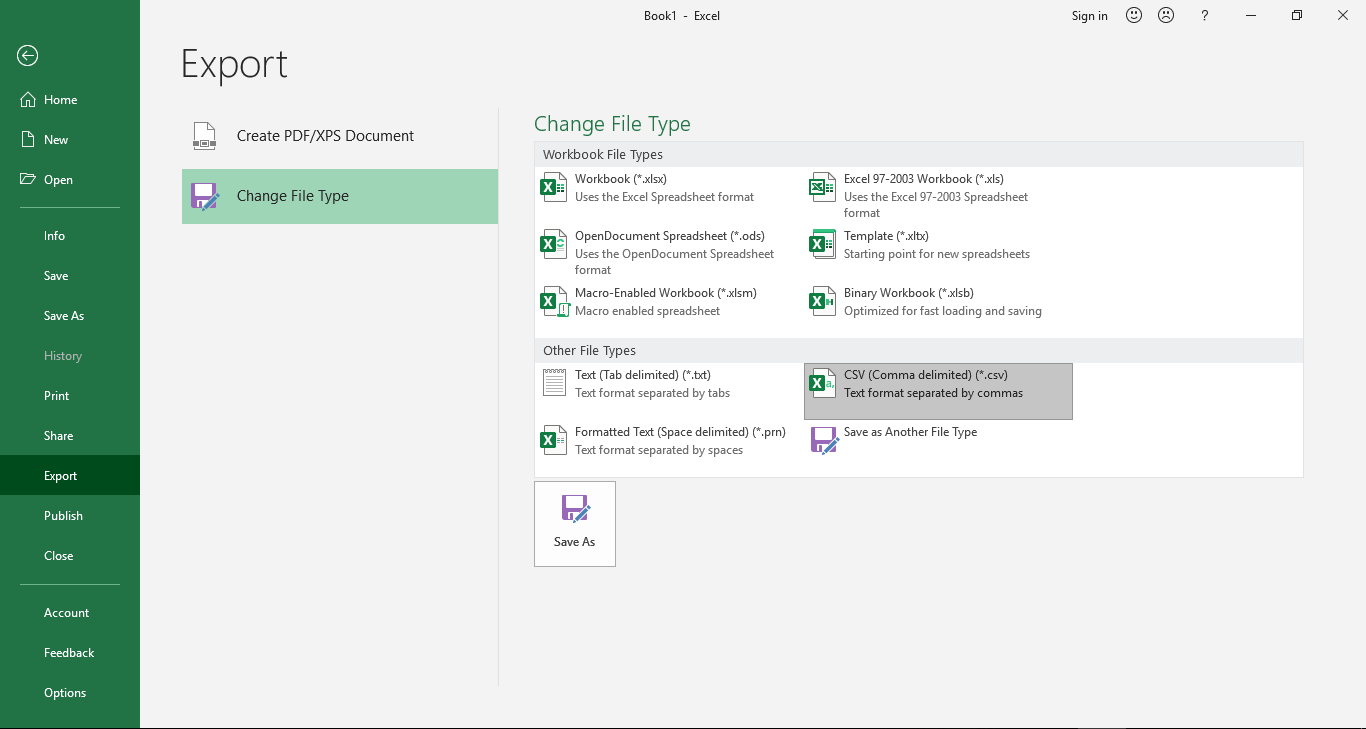
\includegraphics[scale = 0.3]{gambar/csv2.png}
\end{enumerate}

\item Sejarah Library CSV\\
Format CSV(Comma Separated Value) merupakan format ekspor impor yang paling sering digunakan untuk Database dan spreadsheet. CSV menggunakan format standar pada RCF 4180.  Seiring dengan lahirnya bahasa pemrograman python, library mulai dibuat dan dikembangkan sampai akhirnya pada tahun 2003, Kevin Altis dan lainnya telah merilis versi final untuk library Python CSV.

\item Sejarah Library Pandas\\
Pandas (Python Data Analysis Library) adalah alat sebagai analisis data dan struktur bahasa pemrograman python. Pandas Dapat digunakan untuk mengolah data dengan mudah. Pandas diciptakan pada tahun 2008 oleh Wes McKinney dan diperbaharui oleh Sien Chang pada tahun 2010. Inspirasi dari pembuatan pandas muncul pada komunitas yang membutuhkan library khusus untuk analisis data. Salah satu fitur pada pandas adalah Dataframe. Fitur ini membuat kita dapat membaca sebuah file dan membuatnya menjadi table. Banyak file yang dapat dibaca dengan menggunakan Pandas, seperti file .txt, .csv, .tsv, dan masih banyak lagi.

\item Fungsi-Fungsi pada Library CSV\\
\begin{enumerate}
\item Fungsi Reader: untuk membaca isi file CSV dari list.\\
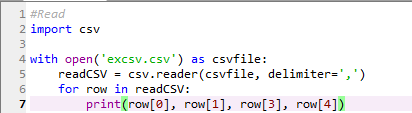
\includegraphics[scale = 0.7]{gambar/csv3.png}
\item DictReader: untuk membaca isi file  CSV dari Dictionary.\\
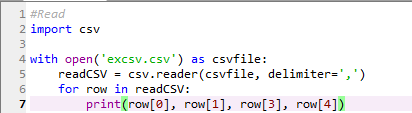
\includegraphics[scale = 0.7]{gambar/csv3.png}
\item Write: untuk menulis file  CSV dari list.\\
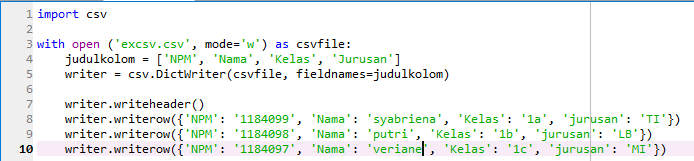
\includegraphics[scale = 0.5]{gambar/csv4.png}
\item DictWrite: untuk menulis file CSV dari Dictionary.\\
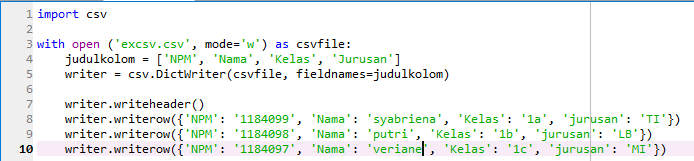
\includegraphics[scale = 0.5]{gambar/csv4.png}
\end{enumerate}

\item Fungsi-Fungsi pada Library Pandas\\
\begin{enumerate}
\item read CSV: Untuk membaca file CSV dan menyimpannya ke DataFrame.\\
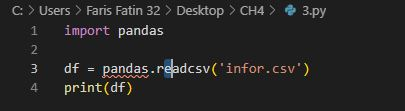
\includegraphics{gambar/csv5.png}
\item to CSV: Untuk menulis file CSV\\
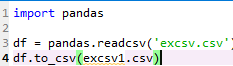
\includegraphics{gambar/csv6.png}
\end{enumerate}

\end{enumerate}

\section{Keterampilan Pemrograman}
\begin{enumerate}
\item Buat csv mode list.\\ 
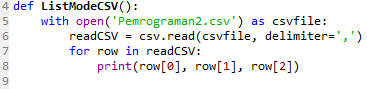
\includegraphics{gambar/csv7.png}
\item Buat csv mode dictionary.\\ 
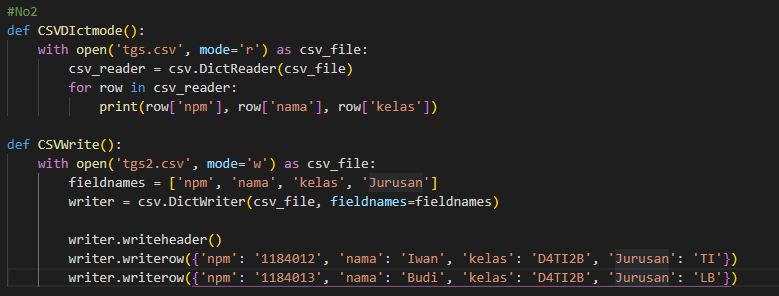
\includegraphics[scale = 0.7]{gambar/csv8.png}
\item Buat fungsi untuk membuka file csv dengan lib pandas mode list.\\
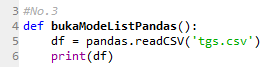
\includegraphics{gambar/csv9.png}
\item Buat fungsi untuk membuka file csv dengan lib pandas mode Dictionary.\\ 
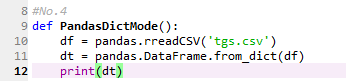
\includegraphics{gambar/csv10.png}
\item Buat fungsi baru di NPM pandas.py untuk mengubah format tanggal menjadi standar dataframe.\\ 
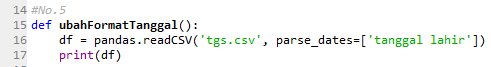
\includegraphics{gambar/csv11.png}
\item Buat fungsi baru di NPM pandas.py untuk mengubah index kolom.\\ 
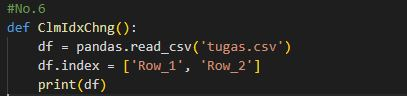
\includegraphics{gambar/csv12.png}
\item Buat fungsi baru di NPM pandas.py untuk mengubah atribut atau nama kolom.\\ 
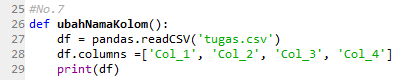
\includegraphics{gambar/csv13.png}
\item Buat program  main.py yang menggunakan library NPM csv.py yang membuat dan membaca file csv.\\ 
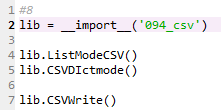
\includegraphics{gambar/csv14.png}
\item Buat program  main2.py yang menggunakan library NPM pandas.py yang membuat dan membaca file csv.\\ 
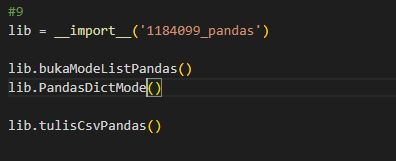
\includegraphics{gambar/csv15.png}

\end{enumerate}
%\begin{enumerate}
%\end{enumerate}

\section{Keterampilan Penanganan Error}
TypeError: NPM2() takes 0 positional arguments but 1 was given \\
solusi: Menambahkan argument pada NPM2().\\

